\documentclass[]{article}
\usepackage{lmodern}
\usepackage{amssymb,amsmath}
\usepackage{ifxetex,ifluatex}
\usepackage{fixltx2e} % provides \textsubscript
\ifnum 0\ifxetex 1\fi\ifluatex 1\fi=0 % if pdftex
  \usepackage[T1]{fontenc}
  \usepackage[utf8]{inputenc}
\else % if luatex or xelatex
  \ifxetex
    \usepackage{mathspec}
  \else
    \usepackage{fontspec}
  \fi
  \defaultfontfeatures{Ligatures=TeX,Scale=MatchLowercase}
\fi
% use upquote if available, for straight quotes in verbatim environments
\IfFileExists{upquote.sty}{\usepackage{upquote}}{}
% use microtype if available
\IfFileExists{microtype.sty}{%
\usepackage{microtype}
\UseMicrotypeSet[protrusion]{basicmath} % disable protrusion for tt fonts
}{}
\usepackage[margin=1in]{geometry}
\usepackage{hyperref}
\hypersetup{unicode=true,
            pdftitle={DATA 606 - Lab 5},
            pdfauthor={Joshua Sturm},
            pdfborder={0 0 0},
            breaklinks=true}
\urlstyle{same}  % don't use monospace font for urls
\usepackage{color}
\usepackage{fancyvrb}
\newcommand{\VerbBar}{|}
\newcommand{\VERB}{\Verb[commandchars=\\\{\}]}
\DefineVerbatimEnvironment{Highlighting}{Verbatim}{commandchars=\\\{\}}
% Add ',fontsize=\small' for more characters per line
\usepackage{framed}
\definecolor{shadecolor}{RGB}{248,248,248}
\newenvironment{Shaded}{\begin{snugshade}}{\end{snugshade}}
\newcommand{\KeywordTok}[1]{\textcolor[rgb]{0.13,0.29,0.53}{\textbf{#1}}}
\newcommand{\DataTypeTok}[1]{\textcolor[rgb]{0.13,0.29,0.53}{#1}}
\newcommand{\DecValTok}[1]{\textcolor[rgb]{0.00,0.00,0.81}{#1}}
\newcommand{\BaseNTok}[1]{\textcolor[rgb]{0.00,0.00,0.81}{#1}}
\newcommand{\FloatTok}[1]{\textcolor[rgb]{0.00,0.00,0.81}{#1}}
\newcommand{\ConstantTok}[1]{\textcolor[rgb]{0.00,0.00,0.00}{#1}}
\newcommand{\CharTok}[1]{\textcolor[rgb]{0.31,0.60,0.02}{#1}}
\newcommand{\SpecialCharTok}[1]{\textcolor[rgb]{0.00,0.00,0.00}{#1}}
\newcommand{\StringTok}[1]{\textcolor[rgb]{0.31,0.60,0.02}{#1}}
\newcommand{\VerbatimStringTok}[1]{\textcolor[rgb]{0.31,0.60,0.02}{#1}}
\newcommand{\SpecialStringTok}[1]{\textcolor[rgb]{0.31,0.60,0.02}{#1}}
\newcommand{\ImportTok}[1]{#1}
\newcommand{\CommentTok}[1]{\textcolor[rgb]{0.56,0.35,0.01}{\textit{#1}}}
\newcommand{\DocumentationTok}[1]{\textcolor[rgb]{0.56,0.35,0.01}{\textbf{\textit{#1}}}}
\newcommand{\AnnotationTok}[1]{\textcolor[rgb]{0.56,0.35,0.01}{\textbf{\textit{#1}}}}
\newcommand{\CommentVarTok}[1]{\textcolor[rgb]{0.56,0.35,0.01}{\textbf{\textit{#1}}}}
\newcommand{\OtherTok}[1]{\textcolor[rgb]{0.56,0.35,0.01}{#1}}
\newcommand{\FunctionTok}[1]{\textcolor[rgb]{0.00,0.00,0.00}{#1}}
\newcommand{\VariableTok}[1]{\textcolor[rgb]{0.00,0.00,0.00}{#1}}
\newcommand{\ControlFlowTok}[1]{\textcolor[rgb]{0.13,0.29,0.53}{\textbf{#1}}}
\newcommand{\OperatorTok}[1]{\textcolor[rgb]{0.81,0.36,0.00}{\textbf{#1}}}
\newcommand{\BuiltInTok}[1]{#1}
\newcommand{\ExtensionTok}[1]{#1}
\newcommand{\PreprocessorTok}[1]{\textcolor[rgb]{0.56,0.35,0.01}{\textit{#1}}}
\newcommand{\AttributeTok}[1]{\textcolor[rgb]{0.77,0.63,0.00}{#1}}
\newcommand{\RegionMarkerTok}[1]{#1}
\newcommand{\InformationTok}[1]{\textcolor[rgb]{0.56,0.35,0.01}{\textbf{\textit{#1}}}}
\newcommand{\WarningTok}[1]{\textcolor[rgb]{0.56,0.35,0.01}{\textbf{\textit{#1}}}}
\newcommand{\AlertTok}[1]{\textcolor[rgb]{0.94,0.16,0.16}{#1}}
\newcommand{\ErrorTok}[1]{\textcolor[rgb]{0.64,0.00,0.00}{\textbf{#1}}}
\newcommand{\NormalTok}[1]{#1}
\usepackage{longtable,booktabs}
\usepackage{graphicx,grffile}
\makeatletter
\def\maxwidth{\ifdim\Gin@nat@width>\linewidth\linewidth\else\Gin@nat@width\fi}
\def\maxheight{\ifdim\Gin@nat@height>\textheight\textheight\else\Gin@nat@height\fi}
\makeatother
% Scale images if necessary, so that they will not overflow the page
% margins by default, and it is still possible to overwrite the defaults
% using explicit options in \includegraphics[width, height, ...]{}
\setkeys{Gin}{width=\maxwidth,height=\maxheight,keepaspectratio}
\IfFileExists{parskip.sty}{%
\usepackage{parskip}
}{% else
\setlength{\parindent}{0pt}
\setlength{\parskip}{6pt plus 2pt minus 1pt}
}
\setlength{\emergencystretch}{3em}  % prevent overfull lines
\providecommand{\tightlist}{%
  \setlength{\itemsep}{0pt}\setlength{\parskip}{0pt}}
\setcounter{secnumdepth}{0}
% Redefines (sub)paragraphs to behave more like sections
\ifx\paragraph\undefined\else
\let\oldparagraph\paragraph
\renewcommand{\paragraph}[1]{\oldparagraph{#1}\mbox{}}
\fi
\ifx\subparagraph\undefined\else
\let\oldsubparagraph\subparagraph
\renewcommand{\subparagraph}[1]{\oldsubparagraph{#1}\mbox{}}
\fi

%%% Use protect on footnotes to avoid problems with footnotes in titles
\let\rmarkdownfootnote\footnote%
\def\footnote{\protect\rmarkdownfootnote}

%%% Change title format to be more compact
\usepackage{titling}

% Create subtitle command for use in maketitle
\newcommand{\subtitle}[1]{
  \posttitle{
    \begin{center}\large#1\end{center}
    }
}

\setlength{\droptitle}{-2em}
  \title{DATA 606 - Lab 5}
  \pretitle{\vspace{\droptitle}\centering\huge}
  \posttitle{\par}
  \author{Joshua Sturm}
  \preauthor{\centering\large\emph}
  \postauthor{\par}
  \predate{\centering\large\emph}
  \postdate{\par}
  \date{October 29, 2017}


\begin{document}
\maketitle

\begin{Shaded}
\begin{Highlighting}[]
\KeywordTok{library}\NormalTok{(ggplot2)}
\end{Highlighting}
\end{Shaded}

\subsection{North Carolina births}\label{north-carolina-births}

In 2004, the state of North Carolina released a large data set
containing information on births recorded in this state. This data set
is useful to researchers studying the relation between habits and
practices of expectant mothers and the birth of their children. We will
work with a random sample of observations from this data set.

\subsection{Exploratory analysis}\label{exploratory-analysis}

Load the \texttt{nc} data set into our workspace.

\begin{Shaded}
\begin{Highlighting}[]
\KeywordTok{load}\NormalTok{(}\StringTok{"more/nc.RData"}\NormalTok{)}
\end{Highlighting}
\end{Shaded}

We have observations on 13 different variables, some categorical and
some numerical. The meaning of each variable is as follows.

\begin{longtable}[]{@{}ll@{}}
\toprule
\begin{minipage}[b]{0.22\columnwidth}\raggedright\strut
variable\strut
\end{minipage} & \begin{minipage}[b]{0.16\columnwidth}\raggedright\strut
description\strut
\end{minipage}\tabularnewline
\midrule
\endhead
\begin{minipage}[t]{0.22\columnwidth}\raggedright\strut
\texttt{fage}\strut
\end{minipage} & \begin{minipage}[t]{0.16\columnwidth}\raggedright\strut
father's age in years.\strut
\end{minipage}\tabularnewline
\begin{minipage}[t]{0.22\columnwidth}\raggedright\strut
\texttt{mage}\strut
\end{minipage} & \begin{minipage}[t]{0.16\columnwidth}\raggedright\strut
mother's age in years.\strut
\end{minipage}\tabularnewline
\begin{minipage}[t]{0.22\columnwidth}\raggedright\strut
\texttt{mature}\strut
\end{minipage} & \begin{minipage}[t]{0.16\columnwidth}\raggedright\strut
maturity status of mother.\strut
\end{minipage}\tabularnewline
\begin{minipage}[t]{0.22\columnwidth}\raggedright\strut
\texttt{weeks}\strut
\end{minipage} & \begin{minipage}[t]{0.16\columnwidth}\raggedright\strut
length of pregnancy in weeks.\strut
\end{minipage}\tabularnewline
\begin{minipage}[t]{0.22\columnwidth}\raggedright\strut
\texttt{premie}\strut
\end{minipage} & \begin{minipage}[t]{0.16\columnwidth}\raggedright\strut
whether the birth was classified as premature (premie) or
full-term.\strut
\end{minipage}\tabularnewline
\begin{minipage}[t]{0.22\columnwidth}\raggedright\strut
\texttt{visits}\strut
\end{minipage} & \begin{minipage}[t]{0.16\columnwidth}\raggedright\strut
number of hospital visits during pregnancy.\strut
\end{minipage}\tabularnewline
\begin{minipage}[t]{0.22\columnwidth}\raggedright\strut
\texttt{marital}\strut
\end{minipage} & \begin{minipage}[t]{0.16\columnwidth}\raggedright\strut
whether mother is \texttt{married} or \texttt{not\ married} at
birth.\strut
\end{minipage}\tabularnewline
\begin{minipage}[t]{0.22\columnwidth}\raggedright\strut
\texttt{gained}\strut
\end{minipage} & \begin{minipage}[t]{0.16\columnwidth}\raggedright\strut
weight gained by mother during pregnancy in pounds.\strut
\end{minipage}\tabularnewline
\begin{minipage}[t]{0.22\columnwidth}\raggedright\strut
\texttt{weight}\strut
\end{minipage} & \begin{minipage}[t]{0.16\columnwidth}\raggedright\strut
weight of the baby at birth in pounds.\strut
\end{minipage}\tabularnewline
\begin{minipage}[t]{0.22\columnwidth}\raggedright\strut
\texttt{lowbirthweight}\strut
\end{minipage} & \begin{minipage}[t]{0.16\columnwidth}\raggedright\strut
whether baby was classified as low birthweight (\texttt{low}) or not
(\texttt{not\ low}).\strut
\end{minipage}\tabularnewline
\begin{minipage}[t]{0.22\columnwidth}\raggedright\strut
\texttt{gender}\strut
\end{minipage} & \begin{minipage}[t]{0.16\columnwidth}\raggedright\strut
gender of the baby, \texttt{female} or \texttt{male}.\strut
\end{minipage}\tabularnewline
\begin{minipage}[t]{0.22\columnwidth}\raggedright\strut
\texttt{habit}\strut
\end{minipage} & \begin{minipage}[t]{0.16\columnwidth}\raggedright\strut
status of the mother as a \texttt{nonsmoker} or a \texttt{smoker}.\strut
\end{minipage}\tabularnewline
\begin{minipage}[t]{0.22\columnwidth}\raggedright\strut
\texttt{whitemom}\strut
\end{minipage} & \begin{minipage}[t]{0.16\columnwidth}\raggedright\strut
whether mom is \texttt{white} or \texttt{not\ white}.\strut
\end{minipage}\tabularnewline
\bottomrule
\end{longtable}

\subsection{Question 1}\label{question-1}

\begin{enumerate}
\def\labelenumi{\arabic{enumi}.}
\tightlist
\item
  What are the cases in this data set? How many cases are there in our
  sample?
\end{enumerate}

\subsubsection{Solution}\label{solution}

\begin{Shaded}
\begin{Highlighting}[]
\KeywordTok{dim}\NormalTok{(nc)}
\end{Highlighting}
\end{Shaded}

\begin{verbatim}
## [1] 1000   13
\end{verbatim}

The cases are births in North Carolina. There are 1000 cases (births) in
our sample.

As a first step in the analysis, we should consider summaries of the
data. This can be done using the \texttt{summary} command:

\begin{Shaded}
\begin{Highlighting}[]
\KeywordTok{summary}\NormalTok{(nc)}
\end{Highlighting}
\end{Shaded}

\begin{verbatim}
##       fage            mage            mature        weeks      
##  Min.   :14.00   Min.   :13   mature mom :133   Min.   :20.00  
##  1st Qu.:25.00   1st Qu.:22   younger mom:867   1st Qu.:37.00  
##  Median :30.00   Median :27                     Median :39.00  
##  Mean   :30.26   Mean   :27                     Mean   :38.33  
##  3rd Qu.:35.00   3rd Qu.:32                     3rd Qu.:40.00  
##  Max.   :55.00   Max.   :50                     Max.   :45.00  
##  NA's   :171                                    NA's   :2      
##        premie        visits            marital        gained     
##  full term:846   Min.   : 0.0   married    :386   Min.   : 0.00  
##  premie   :152   1st Qu.:10.0   not married:613   1st Qu.:20.00  
##  NA's     :  2   Median :12.0   NA's       :  1   Median :30.00  
##                  Mean   :12.1                     Mean   :30.33  
##                  3rd Qu.:15.0                     3rd Qu.:38.00  
##                  Max.   :30.0                     Max.   :85.00  
##                  NA's   :9                        NA's   :27     
##      weight       lowbirthweight    gender          habit    
##  Min.   : 1.000   low    :111    female:503   nonsmoker:873  
##  1st Qu.: 6.380   not low:889    male  :497   smoker   :126  
##  Median : 7.310                               NA's     :  1  
##  Mean   : 7.101                                              
##  3rd Qu.: 8.060                                              
##  Max.   :11.750                                              
##                                                              
##       whitemom  
##  not white:284  
##  white    :714  
##  NA's     :  2  
##                 
##                 
##                 
## 
\end{verbatim}

As you review the variable summaries, consider which variables are
categorical and which are numerical. For numerical variables, are there
outliers? If you aren't sure or want to take a closer look at the data,
make a graph.

Consider the possible relationship between a mother's smoking habit and
the weight of her baby. Plotting the data is a useful first step because
it helps us quickly visualize trends, identify strong associations, and
develop research questions.

\subsection{Question 2}\label{question-2}

\begin{enumerate}
\def\labelenumi{\arabic{enumi}.}
\setcounter{enumi}{1}
\tightlist
\item
  Make a side-by-side boxplot of \texttt{habit} and \texttt{weight}.
  What does the plot highlight about the relationship between these two
  variables?
\end{enumerate}

\paragraph{Solution}\label{solution-1}

\begin{Shaded}
\begin{Highlighting}[]
\KeywordTok{ggplot}\NormalTok{(}\KeywordTok{na.omit}\NormalTok{(nc), }\KeywordTok{aes}\NormalTok{(habit, weight)) }\OperatorTok{+}
\StringTok{  }\KeywordTok{geom_boxplot}\NormalTok{()}
\end{Highlighting}
\end{Shaded}

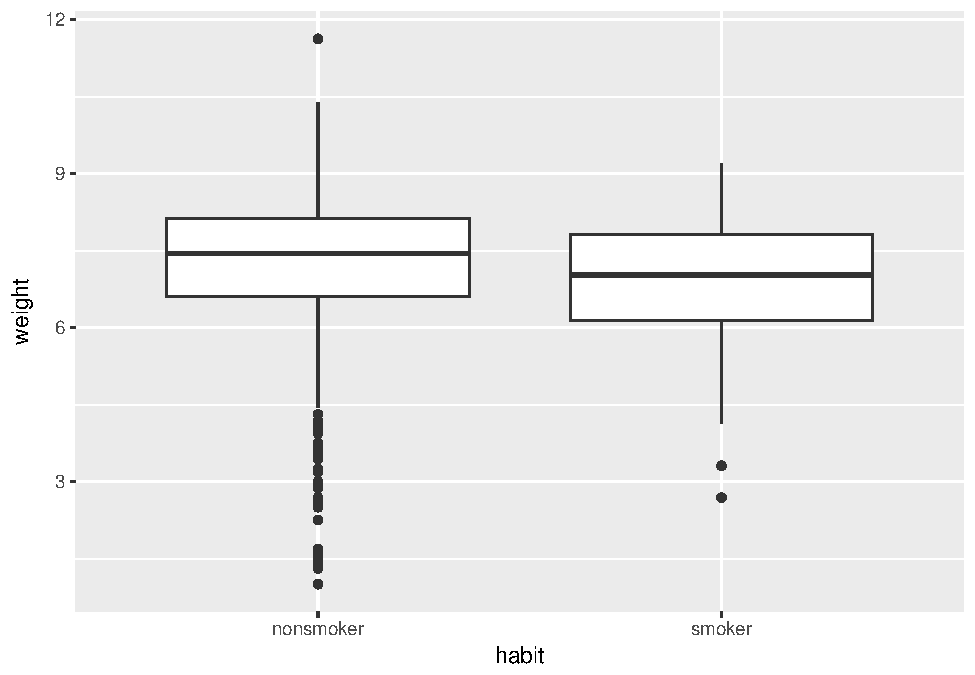
\includegraphics{DATA_606_Lab_5_files/figure-latex/unnamed-chunk-3-1.pdf}
We can see that babies born from non-smoking mothers tend to be heavier
(healthier) than those born from smoking mothers.

The box plots show how the medians of the two distributions compare, but
we can also compare the means of the distributions using the following
function to split the \texttt{weight} variable into the \texttt{habit}
groups, then take the mean of each using the \texttt{mean} function.

\begin{Shaded}
\begin{Highlighting}[]
\KeywordTok{by}\NormalTok{(nc}\OperatorTok{$}\NormalTok{weight, nc}\OperatorTok{$}\NormalTok{habit, mean)}
\end{Highlighting}
\end{Shaded}

\begin{verbatim}
## nc$habit: nonsmoker
## [1] 7.144273
## -------------------------------------------------------- 
## nc$habit: smoker
## [1] 6.82873
\end{verbatim}

There is an observed difference, but is this difference statistically
significant? In order to answer this question we will conduct a
hypothesis test.

\subsection{Inference}\label{inference}

\subsection{Question 3}\label{question-3}

\begin{enumerate}
\def\labelenumi{\arabic{enumi}.}
\setcounter{enumi}{2}
\tightlist
\item
  Check if the conditions necessary for inference are satisfied. Note
  that you will need to obtain sample sizes to check the conditions. You
  can compute the group size using the same \texttt{by} command above
  but replacing \texttt{mean} with \texttt{length}.
\end{enumerate}

\subsubsection{Solution}\label{solution-2}

\begin{Shaded}
\begin{Highlighting}[]
\KeywordTok{by}\NormalTok{(nc}\OperatorTok{$}\NormalTok{weight, nc}\OperatorTok{$}\NormalTok{habit, length)}
\end{Highlighting}
\end{Shaded}

\begin{verbatim}
## nc$habit: nonsmoker
## [1] 873
## -------------------------------------------------------- 
## nc$habit: smoker
## [1] 126
\end{verbatim}

Since \(n = 1000 > 30\), we have a sufficiently large sample.
Furthermore, since this comprises less than 10\% of statewide births, we
can assume that the cases are independent, and the distribution is
nearly normal.

\subsection{Question 4}\label{question-4}

\begin{enumerate}
\def\labelenumi{\arabic{enumi}.}
\setcounter{enumi}{3}
\tightlist
\item
  Write the hypotheses for testing if the average weights of babies born
  to smoking and non-smoking mothers are different.
\end{enumerate}

\subsubsection{Solution}\label{solution-3}

\(H_0: \mu_{s} - \mu_{ns} = 0\). There is no difference in the average
weight of babies born to smoking or nonsmoking mothers.

\(H_A: \mu_{s} - \mu_{ns} \neq 0\). There \emph{is} a difference in the
average weight.

Next, we introduce a new function, \texttt{inference}, that we will use
for conducting hypothesis tests and constructing confidence intervals.

\begin{Shaded}
\begin{Highlighting}[]
\KeywordTok{inference}\NormalTok{(}\DataTypeTok{y =}\NormalTok{ nc}\OperatorTok{$}\NormalTok{weight, }\DataTypeTok{x =}\NormalTok{ nc}\OperatorTok{$}\NormalTok{habit, }\DataTypeTok{est =} \StringTok{"mean"}\NormalTok{, }\DataTypeTok{type =} \StringTok{"ht"}\NormalTok{, }\DataTypeTok{null =} \DecValTok{0}\NormalTok{, }
          \DataTypeTok{alternative =} \StringTok{"twosided"}\NormalTok{, }\DataTypeTok{method =} \StringTok{"theoretical"}\NormalTok{)}
\end{Highlighting}
\end{Shaded}

\begin{verbatim}
## Response variable: numerical, Explanatory variable: categorical
## Difference between two means
## Summary statistics:
## n_nonsmoker = 873, mean_nonsmoker = 7.1443, sd_nonsmoker = 1.5187
## n_smoker = 126, mean_smoker = 6.8287, sd_smoker = 1.3862
\end{verbatim}

\begin{verbatim}
## Observed difference between means (nonsmoker-smoker) = 0.3155
## 
## H0: mu_nonsmoker - mu_smoker = 0 
## HA: mu_nonsmoker - mu_smoker != 0 
## Standard error = 0.134 
## Test statistic: Z =  2.359 
## p-value =  0.0184
\end{verbatim}

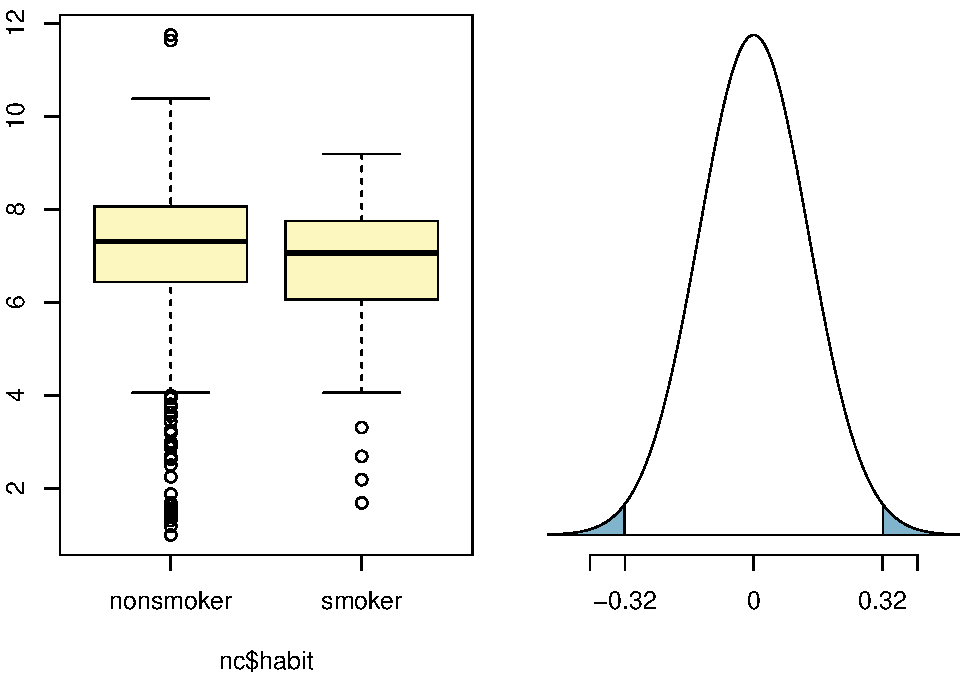
\includegraphics{DATA_606_Lab_5_files/figure-latex/inf-weight-habit-ht-1.pdf}

Let's pause for a moment to go through the arguments of this custom
function. The first argument is \texttt{y}, which is the response
variable that we are interested in: \texttt{nc\$weight}. The second
argument is the explanatory variable, \texttt{x}, which is the variable
that splits the data into two groups, smokers and non-smokers:
\texttt{nc\$habit}. The third argument, \texttt{est}, is the parameter
we're interested in: \texttt{"mean"} (other options are
\texttt{"median"}, or \texttt{"proportion"}.) Next we decide on the
\texttt{type} of inference we want: a hypothesis test (\texttt{"ht"}) or
a confidence interval (\texttt{"ci"}). When performing a hypothesis
test, we also need to supply the \texttt{null} value, which in this case
is \texttt{0}, since the null hypothesis sets the two population means
equal to each other. The \texttt{alternative} hypothesis can be
\texttt{"less"}, \texttt{"greater"}, or \texttt{"twosided"}. Lastly, the
\texttt{method} of inference can be \texttt{"theoretical"} or
\texttt{"simulation"} based.

\subsection{Question 5}\label{question-5}

\begin{enumerate}
\def\labelenumi{\arabic{enumi}.}
\setcounter{enumi}{4}
\tightlist
\item
  Change the \texttt{type} argument to \texttt{"ci"} to construct and
  record a confidence interval for the difference between the weights of
  babies born to smoking and non-smoking mothers.
\end{enumerate}

\subsubsection{Solution}\label{solution-4}

\begin{Shaded}
\begin{Highlighting}[]
\KeywordTok{inference}\NormalTok{(}\DataTypeTok{y =}\NormalTok{ nc}\OperatorTok{$}\NormalTok{weight, }\DataTypeTok{x =}\NormalTok{ nc}\OperatorTok{$}\NormalTok{habit, }\DataTypeTok{est =} \StringTok{"mean"}\NormalTok{, }\DataTypeTok{type =} \StringTok{"ci"}\NormalTok{, }\DataTypeTok{null =} \DecValTok{0}\NormalTok{, }
          \DataTypeTok{alternative =} \StringTok{"twosided"}\NormalTok{, }\DataTypeTok{method =} \StringTok{"theoretical"}\NormalTok{)}
\end{Highlighting}
\end{Shaded}

\begin{verbatim}
## Response variable: numerical, Explanatory variable: categorical
## Difference between two means
## Summary statistics:
## n_nonsmoker = 873, mean_nonsmoker = 7.1443, sd_nonsmoker = 1.5187
## n_smoker = 126, mean_smoker = 6.8287, sd_smoker = 1.3862
\end{verbatim}

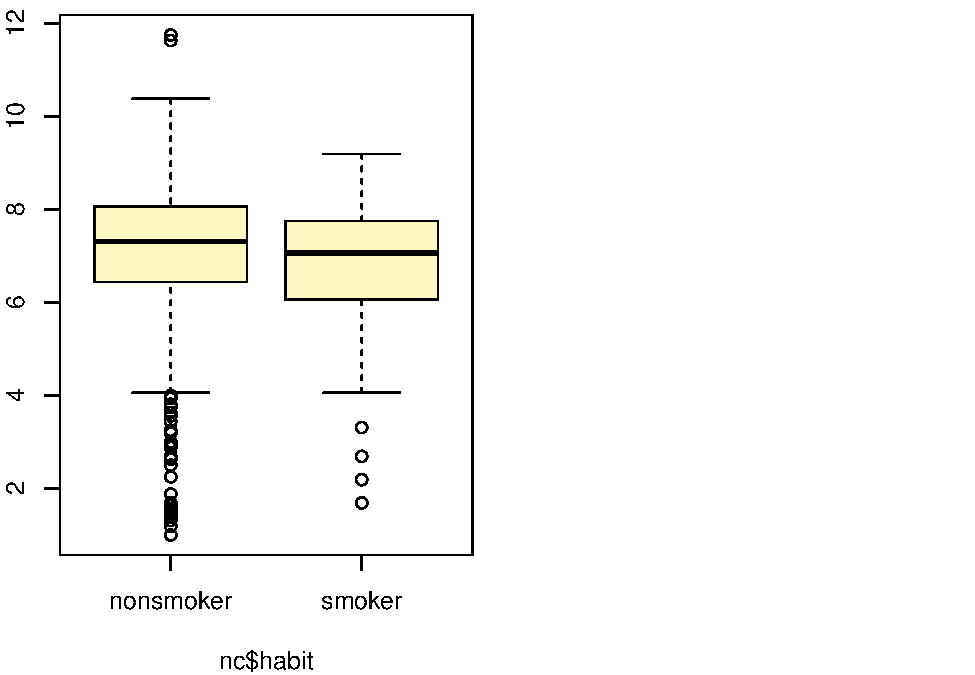
\includegraphics{DATA_606_Lab_5_files/figure-latex/unnamed-chunk-5-1.pdf}

\begin{verbatim}
## Observed difference between means (nonsmoker-smoker) = 0.3155
## 
## Standard error = 0.1338 
## 95 % Confidence interval = ( 0.0534 , 0.5777 )
\end{verbatim}

By default the function reports an interval for
(\(\mu_{nonsmoker} - \mu_{smoker}\)) . We can easily change this order
by using the \texttt{order} argument:

\begin{Shaded}
\begin{Highlighting}[]
\KeywordTok{inference}\NormalTok{(}\DataTypeTok{y =}\NormalTok{ nc}\OperatorTok{$}\NormalTok{weight, }\DataTypeTok{x =}\NormalTok{ nc}\OperatorTok{$}\NormalTok{habit, }\DataTypeTok{est =} \StringTok{"mean"}\NormalTok{, }\DataTypeTok{type =} \StringTok{"ci"}\NormalTok{, }\DataTypeTok{null =} \DecValTok{0}\NormalTok{, }
          \DataTypeTok{alternative =} \StringTok{"twosided"}\NormalTok{, }\DataTypeTok{method =} \StringTok{"theoretical"}\NormalTok{, }
          \DataTypeTok{order =} \KeywordTok{c}\NormalTok{(}\StringTok{"smoker"}\NormalTok{,}\StringTok{"nonsmoker"}\NormalTok{))}
\end{Highlighting}
\end{Shaded}

\begin{verbatim}
## Response variable: numerical, Explanatory variable: categorical
## Difference between two means
## Summary statistics:
## n_smoker = 126, mean_smoker = 6.8287, sd_smoker = 1.3862
## n_nonsmoker = 873, mean_nonsmoker = 7.1443, sd_nonsmoker = 1.5187
\end{verbatim}

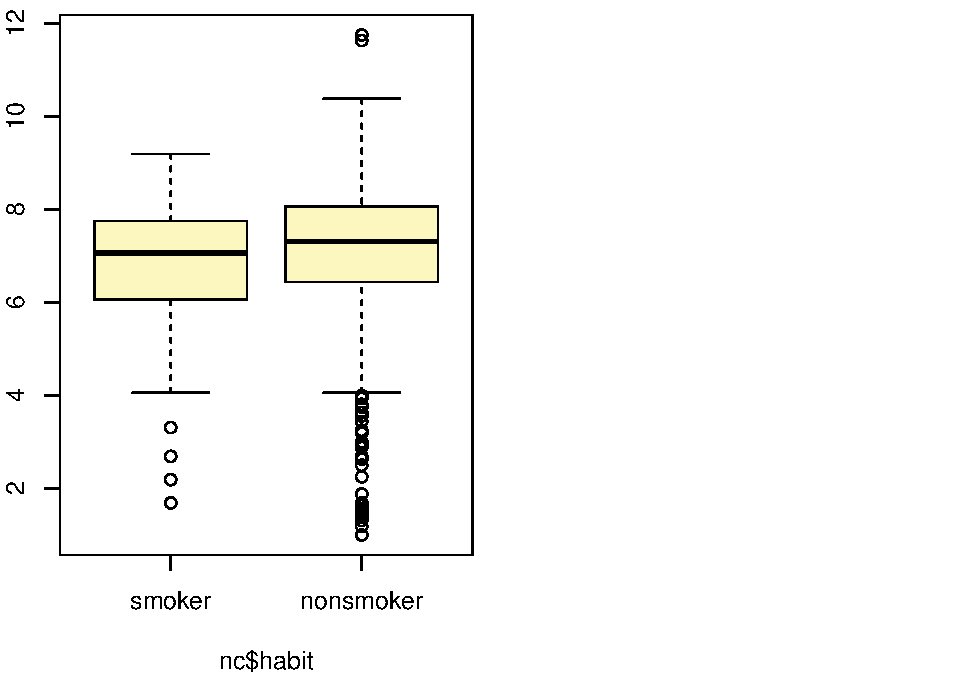
\includegraphics{DATA_606_Lab_5_files/figure-latex/inf-weight-habit-ci-1.pdf}

\begin{verbatim}
## Observed difference between means (smoker-nonsmoker) = -0.3155
## 
## Standard error = 0.1338 
## 95 % Confidence interval = ( -0.5777 , -0.0534 )
\end{verbatim}

\begin{center}\rule{0.5\linewidth}{\linethickness}\end{center}

\subsection{On your own}\label{on-your-own}

\subsection{1}\label{section}

Calculate a 95\% confidence interval for the average length of
pregnancies (\texttt{weeks}) and interpret it in context. Note that
since you're doing inference on a single population parameter, there is
no explanatory variable, so you can omit the \texttt{x} variable from
the function.

\subsubsection{Solution}\label{solution-5}

\begin{Shaded}
\begin{Highlighting}[]
\KeywordTok{inference}\NormalTok{(}\DataTypeTok{y =}\NormalTok{ nc}\OperatorTok{$}\NormalTok{weeks, }\DataTypeTok{est =} \StringTok{"mean"}\NormalTok{, }\DataTypeTok{type =} \StringTok{"ci"}\NormalTok{, }\DataTypeTok{null =} \DecValTok{0}\NormalTok{, }
          \DataTypeTok{alternative =} \StringTok{"twosided"}\NormalTok{, }\DataTypeTok{method =} \StringTok{"theoretical"}\NormalTok{)}
\end{Highlighting}
\end{Shaded}

\begin{verbatim}
## Single mean 
## Summary statistics:
\end{verbatim}

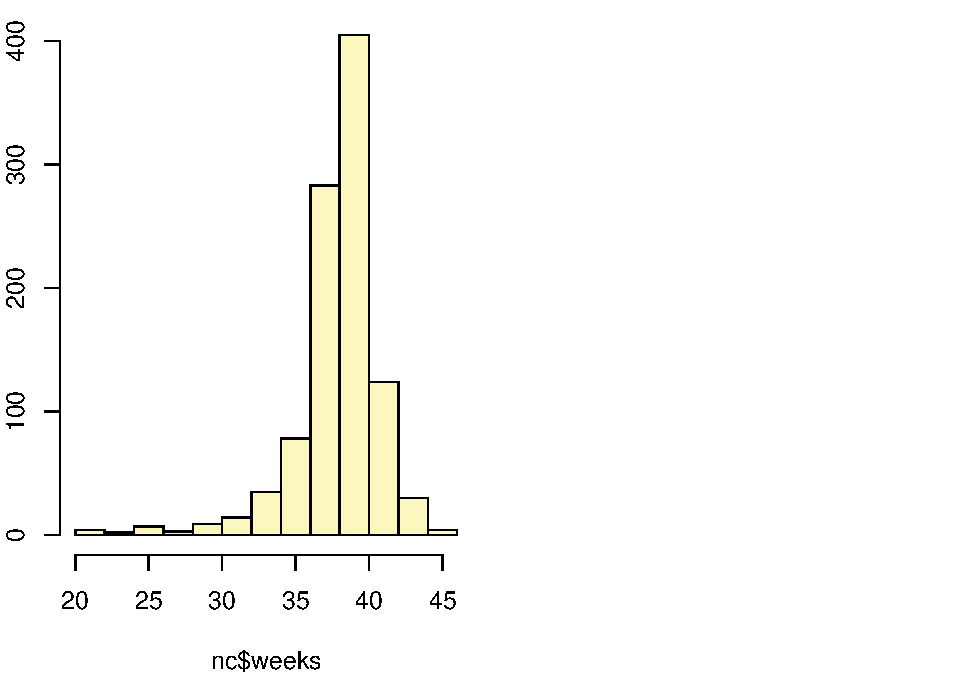
\includegraphics{DATA_606_Lab_5_files/figure-latex/unnamed-chunk-6-1.pdf}

\begin{verbatim}
## mean = 38.3347 ;  sd = 2.9316 ;  n = 998 
## Standard error = 0.0928 
## 95 % Confidence interval = ( 38.1528 , 38.5165 )
\end{verbatim}

We are 95\% confident that the average duration for births in North
Carolina is between 38.1528 and 38.5165 weeks.

\subsection{2}\label{section-1}

Calculate a new confidence interval for the same parameter at the 90\%
confidence level. You can change the confidence level by adding a new
argument to the function: \texttt{conflevel\ =\ 0.90}.

\subsubsection{Solution}\label{solution-6}

\begin{Shaded}
\begin{Highlighting}[]
\KeywordTok{inference}\NormalTok{(}\DataTypeTok{y =}\NormalTok{ nc}\OperatorTok{$}\NormalTok{weeks, }\DataTypeTok{est =} \StringTok{"mean"}\NormalTok{, }\DataTypeTok{type =} \StringTok{"ci"}\NormalTok{, }\DataTypeTok{null =} \DecValTok{0}\NormalTok{, }
          \DataTypeTok{alternative =} \StringTok{"twosided"}\NormalTok{, }\DataTypeTok{method =} \StringTok{"theoretical"}
\NormalTok{          ,}\DataTypeTok{conflevel =} \FloatTok{0.90}\NormalTok{)}
\end{Highlighting}
\end{Shaded}

\begin{verbatim}
## Single mean 
## Summary statistics:
\end{verbatim}

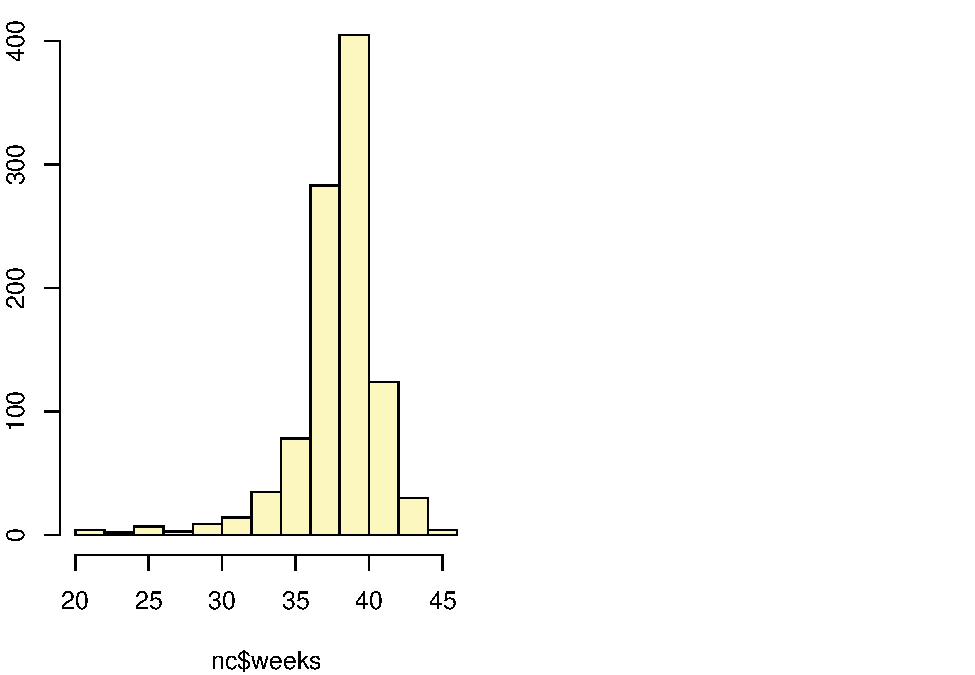
\includegraphics{DATA_606_Lab_5_files/figure-latex/unnamed-chunk-7-1.pdf}

\begin{verbatim}
## mean = 38.3347 ;  sd = 2.9316 ;  n = 998 
## Standard error = 0.0928 
## 90 % Confidence interval = ( 38.182 , 38.4873 )
\end{verbatim}

We are 90\% confident that the average duration for births in North
Carolina is between 38.182 and 38.4873 weeks. Since we have a lower
confidence standard, we can use a smaller interval.

\subsection{3}\label{section-2}

Conduct a hypothesis test evaluating whether the average weight gained
by younger mothers is different than the average weight gained by mature
mothers.

\subsubsection{Solution}\label{solution-7}

\(H_0: \mu_{\text{weightyoung}} - \mu_{\text{weightmature}} = 0\). There
is no difference in weight gain between younger and older mothers.

\(H_A: \mu_{\text{weightyoung}} - \mu_{\text{weightmature}} \neq 0\).
There is a difference in average weight gain.

\begin{Shaded}
\begin{Highlighting}[]
\KeywordTok{inference}\NormalTok{(}\DataTypeTok{y =}\NormalTok{ nc}\OperatorTok{$}\NormalTok{gained, }\DataTypeTok{x =}\NormalTok{ nc}\OperatorTok{$}\NormalTok{mature, }\DataTypeTok{est =} \StringTok{"mean"}\NormalTok{, }\DataTypeTok{type =} \StringTok{"ht"}\NormalTok{, }\DataTypeTok{null =} \DecValTok{0}\NormalTok{, }
          \DataTypeTok{alternative =} \StringTok{"twosided"}\NormalTok{, }\DataTypeTok{method =} \StringTok{"theoretical"}\NormalTok{, }
          \DataTypeTok{order =} \KeywordTok{c}\NormalTok{(}\StringTok{"younger mom"}\NormalTok{, }\StringTok{"mature mom"}\NormalTok{))}
\end{Highlighting}
\end{Shaded}

\begin{verbatim}
## Response variable: numerical, Explanatory variable: categorical
## Difference between two means
## Summary statistics:
## n_younger mom = 844, mean_younger mom = 30.5604, sd_younger mom = 14.3469
## n_mature mom = 129, mean_mature mom = 28.7907, sd_mature mom = 13.4824
\end{verbatim}

\begin{verbatim}
## Observed difference between means (younger mom-mature mom) = 1.7697
## 
## H0: mu_younger mom - mu_mature mom = 0 
## HA: mu_younger mom - mu_mature mom != 0 
## Standard error = 1.286 
## Test statistic: Z =  1.376 
## p-value =  0.1686
\end{verbatim}

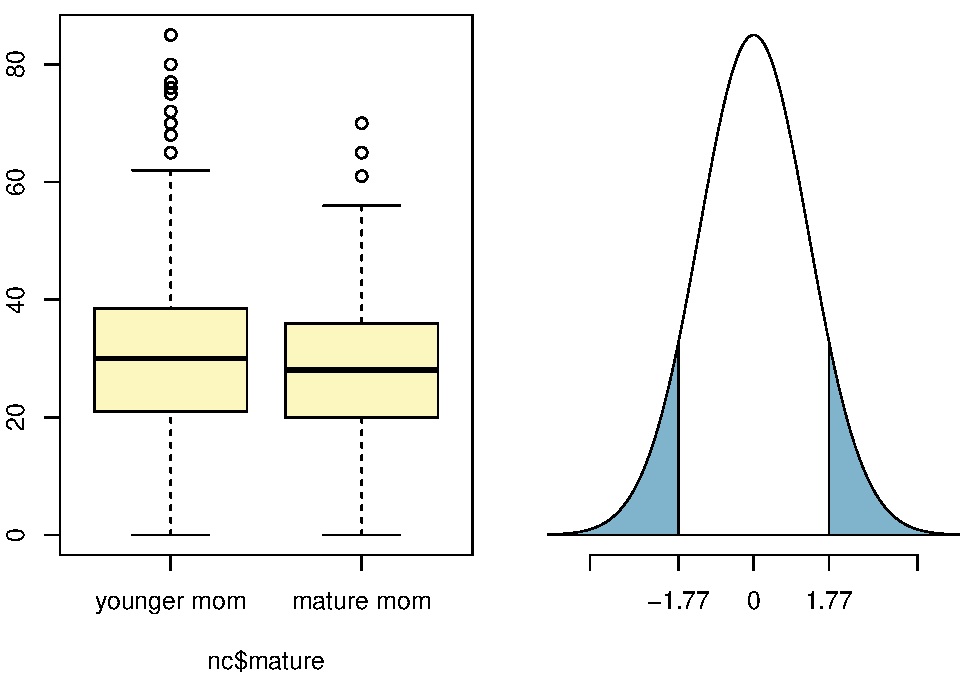
\includegraphics{DATA_606_Lab_5_files/figure-latex/unnamed-chunk-8-1.pdf}
Since \(p = 0.1686 > p = 0.05,\) we accept the null hypothesis, and
conclude there is no significant difference in weight gained during
pregnancy between younger and older mothers.

\subsection{4}\label{section-3}

Now, a non-inference task: Determine the age cutoff for younger and
mature mothers. Use a method of your choice, and explain how your method
works.

\subsubsection{Solution}\label{solution-8}

\begin{Shaded}
\begin{Highlighting}[]
\KeywordTok{by}\NormalTok{(nc}\OperatorTok{$}\NormalTok{mage, nc}\OperatorTok{$}\NormalTok{mature, summary)}
\end{Highlighting}
\end{Shaded}

\begin{verbatim}
## nc$mature: mature mom
##    Min. 1st Qu.  Median    Mean 3rd Qu.    Max. 
##   35.00   35.00   37.00   37.18   38.00   50.00 
## -------------------------------------------------------- 
## nc$mature: younger mom
##    Min. 1st Qu.  Median    Mean 3rd Qu.    Max. 
##   13.00   21.00   25.00   25.44   30.00   34.00
\end{verbatim}

The age interval for younger mothers is (13, 34), and (35, 50) for
mature mothers.

\subsection{5}\label{section-4}

Pick a pair of numerical and categorical variables and come up with a
research question evaluating the relationship between these variables.
Formulate the question in a way that it can be answered using a
hypothesis test and/or a confidence interval. Answer your question using
the \texttt{inference} function, report the statistical results, and
also provide an explanation in plain language.

\subsubsection{}\label{section-5}

Is there a correlation between \texttt{age} of the mother, and
likelihood to give birth \texttt{prematurely}?

\(H_0: \mu_{\text{youngmother}} - \mu_{\text{maturemother}} = 0\). Age
does not affect the likelihood of giving birth prematurely.

\(H_A: \mu_{\text{youngmother}} - \mu_{\text{maturemother}} \neq 0\).
Age does affect the likelihood of giving birth prematurely.

\begin{Shaded}
\begin{Highlighting}[]
\KeywordTok{inference}\NormalTok{(}\DataTypeTok{y =}\NormalTok{ nc}\OperatorTok{$}\NormalTok{mage, }\DataTypeTok{x =}\NormalTok{ nc}\OperatorTok{$}\NormalTok{premie, }\DataTypeTok{est =} \StringTok{"mean"}\NormalTok{, }\DataTypeTok{type =} \StringTok{"ht"}\NormalTok{, }\DataTypeTok{null =} \DecValTok{0}\NormalTok{,}
          \DataTypeTok{alternative =} \StringTok{"twosided"}\NormalTok{, }\DataTypeTok{method =} \StringTok{"theoretical"}\NormalTok{)}
\end{Highlighting}
\end{Shaded}

\begin{verbatim}
## Response variable: numerical, Explanatory variable: categorical
## Difference between two means
## Summary statistics:
## n_full term = 846, mean_full term = 27, sd_full term = 6.1444
## n_premie = 152, mean_premie = 26.875, sd_premie = 6.533
\end{verbatim}

\begin{verbatim}
## Observed difference between means (full term-premie) = 0.125
## 
## H0: mu_full term - mu_premie = 0 
## HA: mu_full term - mu_premie != 0 
## Standard error = 0.57 
## Test statistic: Z =  0.219 
## p-value =  0.8266
\end{verbatim}

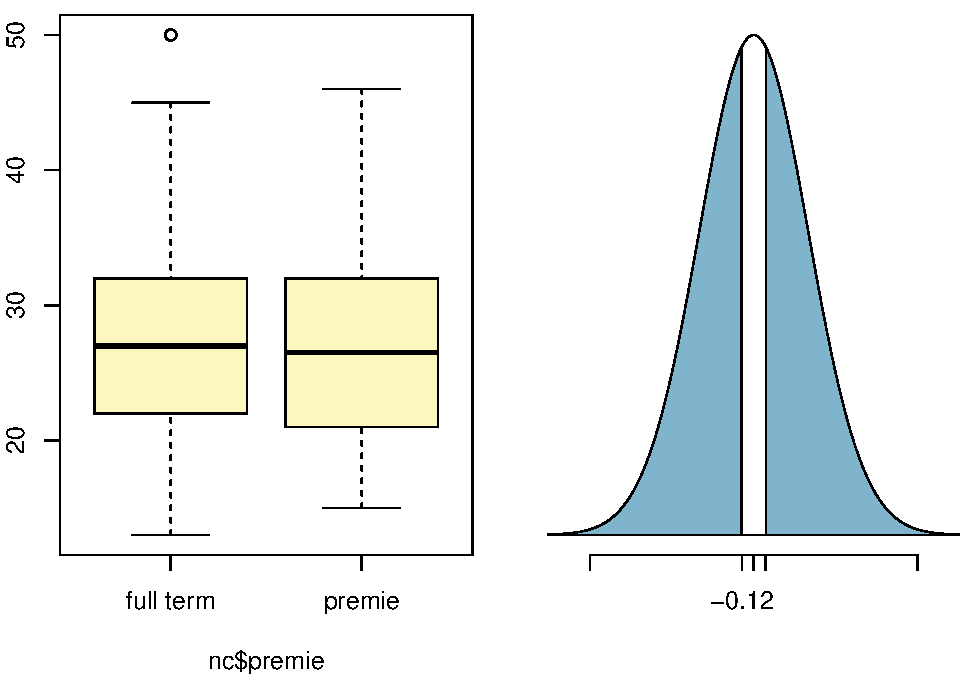
\includegraphics{DATA_606_Lab_5_files/figure-latex/unnamed-chunk-10-1.pdf}

Since \(p = 0.8266 > p = 0.05\), we accept the null hypothesis, and
conclude that the age of the mother does not affect the chance of giving
birth prematurely.


\end{document}
